% ----------------------------------------------------
% Literature Review
% ----------------------------------------------------
\documentclass[class=report,11pt,crop=false]{standalone}
% Page geometry
\usepackage[a4paper,margin=20mm,top=25mm,bottom=25mm]{geometry}

% Font choice
\usepackage{lmodern}

\usepackage{lipsum}

% Use IEEE bibliography style
\bibliographystyle{IEEEtran}

% Line spacing
\usepackage{setspace}
\setstretch{1.20}

% Ensure UTF8 encoding
\usepackage[utf8]{inputenc}

% Language standard (not too important)
\usepackage[english]{babel}

% Skip a line in between paragraphs
\usepackage{parskip}

% For the creation of dummy text
\usepackage{blindtext}

% Math
\usepackage{amsmath}

% Header & Footer stuff
\usepackage{fancyhdr}
\pagestyle{fancy}
\fancyhead{}
\fancyhead[R]{\nouppercase{\rightmark}}
\fancyfoot{}
\fancyfoot[C]{\thepage}
\renewcommand{\headrulewidth}{0.0pt}
\renewcommand{\footrulewidth}{0.0pt}
\setlength{\headheight}{13.6pt}

% Epigraphs
\usepackage{epigraph}
\setlength\epigraphrule{0pt}
\setlength{\epigraphwidth}{0.65\textwidth}

% Colour
\usepackage{color}
\usepackage[usenames,dvipsnames]{xcolor}

% Hyperlinks & References
\usepackage{hyperref}
\definecolor{linkColour}{RGB}{77,71,179}
\hypersetup{
    colorlinks=true,
    linkcolor=linkColour,
    filecolor=linkColour,
    urlcolor=linkColour,
    citecolor=linkColour,
}
\urlstyle{same}

% Automatically correct front-side quotes
\usepackage[autostyle=false, style=ukenglish]{csquotes}
\MakeOuterQuote{"}

% Graphics
\usepackage{graphicx}
\graphicspath{{Images/}{../Images/}}
\usepackage{makecell}
\usepackage{transparent}

% SI units
\usepackage{siunitx}

% Microtype goodness
\usepackage{microtype}

% Listings
\usepackage[T1]{fontenc}
\usepackage{listings}
\usepackage[scaled=0.8]{DejaVuSansMono}

% Custom colours for listings
\definecolor{backgroundColour}{RGB}{250,250,250}
\definecolor{commentColour}{RGB}{73, 175, 102}
\definecolor{identifierColour}{RGB}{196, 19, 66}
\definecolor{stringColour}{RGB}{252, 156, 30}
\definecolor{keywordColour}{RGB}{50, 38, 224}
\definecolor{lineNumbersColour}{RGB}{127,127,127}
\lstset{
  language=Matlab,
  captionpos=b,
  aboveskip=15pt,belowskip=10pt,
  backgroundcolor=\color{backgroundColour},
  basicstyle=\ttfamily,%\footnotesize,        % the size of the fonts that are used for the code
  breakatwhitespace=false,         % sets if automatic breaks should only happen at whitespace
  breaklines=true,                 % sets automatic line breaking
  postbreak=\mbox{\textcolor{red}{$\hookrightarrow$}\space},
  commentstyle=\color{commentColour},    % comment style
  identifierstyle=\color{identifierColour},
  stringstyle=\color{stringColour},
   keywordstyle=\color{keywordColour},       % keyword style
  %escapeinside={\%*}{*)},          % if you want to add LaTeX within your code
  extendedchars=true,              % lets you use non-ASCII characters; for 8-bits encodings only, does not work with UTF-8
  frame=single,	                   % adds a frame around the code
  keepspaces=true,                 % keeps spaces in text, useful for keeping indentation of code (possibly needs columns=flexible)
  morekeywords={*,...},            % if you want to add more keywords to the set
  numbers=left,                    % where to put the line-numbers; possible values are (none, left, right)
  numbersep=5pt,                   % how far the line-numbers are from the code
  numberstyle=\tiny\color{lineNumbersColour}, % the style that is used for the line-numbers
  rulecolor=\color{black},         % if not set, the frame-color may be changed on line-breaks within not-black text (e.g. comments (green here))
  showspaces=false,                % show spaces everywhere adding particular underscores; it overrides 'showstringspaces'
  showstringspaces=false,          % underline spaces within strings only
  showtabs=false,                  % show tabs within strings adding particular underscores
  stepnumber=1,                    % the step between two line-numbers. If it's 1, each line will be numbered
  tabsize=2,	                   % sets default tabsize to 2 spaces
  %title=\lstname                   % show the filename of files included with \lstinputlisting; also try caption instead of title
}

% Caption stuff
\usepackage[hypcap=true, justification=centering]{caption}
\usepackage{subcaption}

% Glossary package
% \usepackage[acronym]{glossaries}
\usepackage{glossaries-extra}
\setabbreviationstyle[acronym]{long-short}

% For Proofs & Theorems
\usepackage{amsthm}

% Maths symbols
\usepackage{amssymb}
\usepackage{mathrsfs}
\usepackage{mathtools}

% For algorithms
\usepackage[]{algorithm2e}

% Spacing stuff
\setlength{\abovecaptionskip}{5pt plus 3pt minus 2pt}
\setlength{\belowcaptionskip}{5pt plus 3pt minus 2pt}
\setlength{\textfloatsep}{10pt plus 3pt minus 2pt}
\setlength{\intextsep}{15pt plus 3pt minus 2pt}

% For aligning footnotes at bottom of page, instead of hugging text
\usepackage[bottom]{footmisc}

% Add LoF, Bib, etc. to ToC
\usepackage[nottoc]{tocbibind}

% SI
\usepackage{siunitx}

% For removing some whitespace in Chapter headings etc
\usepackage{etoolbox}
\makeatletter
\patchcmd{\@makechapterhead}{\vspace*{50\p@}}{\vspace*{-10pt}}{}{}%
\patchcmd{\@makeschapterhead}{\vspace*{50\p@}}{\vspace*{-10pt}}{}{}%
\makeatother

\begin{document}
\ifstandalone
\tableofcontents
\fi
% ----------------------------------------------------
\chapter{Literature Review \label{ch:literature}}
\vspace{0.5cm}
% ----------------------------------------------------

\section{Introduction}
In this section we will discuss articles relating to weighing of birds, remote data interfacing, and the behaviour of birds (focusing on Red Winged Starlings). These are all in pursuit of getting insights into the birds and possible technologies available to solve the presented problem.

\section{The Importance of Monitoring Avian Weight Changes}
According to Clark, “Weight summarizes the total biomass of an individual and is probably the most convenient standard of energetic comparisons.” \cite{ClarckWeights}, which emphasizes how valuable the weight data of an individual bird can be. Baldwin and Kendeigh state that “The weight of birds and the variations and fluctuations of these weights furnish criteria of considerable importance in the understanding of the physiological and ecological reactions of the bird as a living organism \cite{BaldwinWeights}, which further establishes how important the tracking of an individual bird’s weight data can be. Both of these statements cement how valuable weight data can be for ornithologists studying individual birds.

Clark goes on to say, “Weights have been used in analyses of the factors that influence differences in species diversity between communities.” \cite{ClarckWeights}. They also state that “Weights and census data have often been combined to calculate the total biomass of a particular species or group of species in an area”. These statements add that weight data could also be invaluable for the analysis of an entire community of birds as opposed to just monitoring individuals.

\section{Current Weighing Methods}
This section explores and evaluates the different weighing methods used in ornithological research today with a focus on smaller birds (those weighing less than 100g).

\subsection{Spring Scales}
Spring scales measure weight based on the extension of a spring when a force (the weight of the bird) is applied. Their main advantage, as described by Manolis \cite{manoils2024simple}, is that they are “relatively inexpensive and sufficiently portable to suffice for short-term field project[s]”. However, within the same study, the scale was only accurate to within 0,5g and when smaller birds can weigh less than 50g, spring scales may lack the precision for such research applications. Readings can also be influenced by factors such as calibration drift.

\subsection{Electronic Scales}
Electronic scales utilize load cells or strain gauges to convert the weight of the bird into an electronic signal, which can then be displayed on a digital screen. These scales offer precise measurements and are commonly used in both laboratory and field settings. This is shown in Carpenter et al. \cite{carpenter1983weight} paper where they were able to improve the precision of their measurements from 0,05g to 0,01g by simply replacing their spring scales with electronic ones. Another advantage over spring scales is that they do not have to be recalibrated after moving \cite{carpenter1983weight} and they tend to come with features such as taring functions to account for container weight or bird movements.

\subsection{Perching Scales}
Perching scales integrate a weighing platform into an artificial perch or nest. In Poole and Shoukimas’ \cite{poole1982scale} study, birds landing on perch would deflect a transducer (a metal beam with 4 strain gauges bonded to it), thus generating an electronic signal. Reid et al. \cite{reid1999measurement} used artificial nests rigged with a load cell in much the same way. In both studies, these electronic signals would then be recorded via some kind of electronic storage medium. This meant the birds could be weighed remotely, which minimizes stress and reduces the risk of injury, making perching scales particularly useful for long-term monitoring studies or behavioural observations. However, for such long-term studies, researchers would need to keep track of a large number of birds, which would also result in a large amount of data that needs to be stored.

Manolis \cite{manoils2024simple} provides a solution to these issues by urging other researchers to make use of telemetric equipment. One such technology is Radio Frequency Identification (RFID) which enables researchers to track individual birds and record their weight automatically. Wang et al. \cite{wang2019rfid} made use of RFID by attaching two transponders to each bird, which would be detected by antennas placed under the perches. When a tagged bird interacts with the RFID reader, its unique identifier and weight are recorded electronically. This makes the data much easier to organise. It also reduces the volume of data as the weight is only taken when the birds are on top of the perch, allowing researchers to collect data on a larger scale. 


\section{Data Transmission and User Interface}
The method that the FitzPatrick Institute currently have for reading the bird weight is having someone go up to the scale and read off screen on the scale. Then they record the weight into \textit{Cybertracker}, a mobile app for collecting field data \cite{cybertracker}. The app creates an Excel spreadsheet for them to analyze. 
They need a way to access that data remotely; or perhaps, a way to send that data directly to the Cybertracker app. We need to figure out two things: where do we want the data to be directly sent to, and using which protocol.

We investigated different options for transmitting data from a microprocessor. In a comparative performance study by Eridani et al., three protocols were compared: Bluetooth, Wi-Fi direct, and ESP-NOW ("a new protocol that allows multiple devices to communicate with each other without the use of Wi-Fi, with low power consumption" \cite{comparitiveEspnow}). Five metrics were used in the tests: maximum range, transmission speed, latency, power usage, and signal resistance to obstructions \cite{comparitiveEspnow}. A brief summary of the performance of each protocol is shown below in Figure \ref{fig:performance}.
\begin{figure}[h]
	\centering
	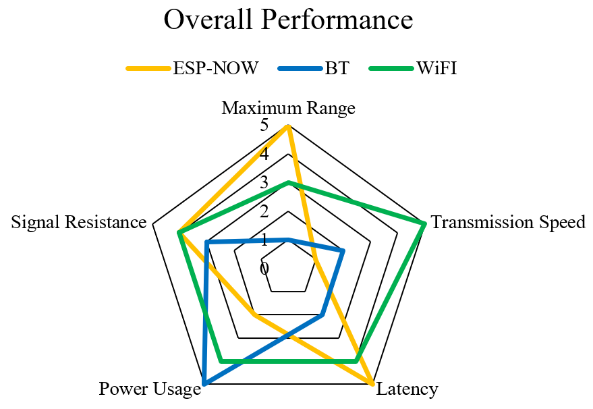
\includegraphics[width=0.7\linewidth]{Figures/performance}
	\caption{Overall Performance of each Protocol \cite{comparitiveEspnow}}
	\label{fig:performance}
\end{figure}

ESP-NOW performs best in range and latency; Bluetooth in power usage; and Wi-Fi in transmission speed. In our context, power usage would be most important. Bluetooth seems to provide sufficient range and speed.
The problem with this; however, is that connecting the system to the user's phone requires effort and perhaps expertise that the user may not have. In this case, connecting the system to the internet may be a better option (if internet connection is available, i.e. if \textit{eduroam} is in range). 

Budoyo and Andriana used the internet when designing a prototype of a digital scale to measure the weight of onions. \cite{iot}. They interfaced the microcontroller (an  ATMega2560) to the internet using an ESP8266 Wi-Fi module. The weight data is sent to a website where it is stored in a database. A database is useful in creating an Excel spreadsheet with many fields which is the end product that the client requires.

\section{Power supply}	
Traditional weighing scales have historically relied on either battery or electric power sources for operation. Battery-powered scales utilize internal batteries, commonly alkaline or lithium-ion, to supply the necessary electrical power. This section will discuss the different types of power supplies available for bird scales, power limitations what type of power source our design will use.

\subsection{Wall Power}
For indoor scales, which are in a fixed environment, the electric-type scales are directly connected to a power source via a cord, typically drawing from AC power provided by a wall outlet. These are the type of scales used in laboratories and residential environments. 

\subsection{Energy Harvesting}
One other method researchers use in low powered bird scales is Energy Harvesting (EH). Energy Harvesting is used to extend the lifespan of the scale and sensing devices, however the process is not always effective \cite{EnergyHarvesting}. An example of energy harvesting would be using wind or solar as a power source to the scale device. This concept is mostly useful in situations where the scale is scale device is left into the environment for data capture, and only accessed after a prolonged period of time. In the case of our design, Sally will be able to access the designed scale at any time she would desire.  

It is worth noting that low-power weighing scales are an existing topic, where in some cases there are scales and sensors that are able to input environmental measurements, read and communicate the data in real time \cite{ImageBased}. As discussed in Section 2.3 above, our design will use Wifi to communicate data to the researcher. The scale will use an alkaline battery power source. Alkaline batteries typically have a lifespan of 5 to 10 years, with an operational voltage range of between 1.5-1.6V. The batteries can operate extreme temperature conditions, typically between -20 to 54 degrees celsius.

\subsection{Limitations}
The reliance on electrical power poses serious constraints, particularly in terms of mobility. This limitation becomes pronounced in specialized applications such as bird weighing scales, especially is weighing of birds such as starlings, which are very mobile. A better solution is to use a rechargeable battery source, such as the alkaline batteries mentioned above. Environmental conditions also pose a risk to the battery lifespan. Solar panels can pose collision risks for birds, particularly if the panels are highly reflective. Some birds may collide with solar panels while flying, leading to injury or mortality. Henceforth, using solar panels for our design is ruled out.
 

\section{Challenges and Considerations}
While modern weighing methods offer significant advantages in terms of accuracy, convenience, and animal welfare, researchers must consider several factors when selecting the most appropriate technique for their study.

\subsection{Size and Species}
The size and behaviour of the target bird species may influence the suitability of different weighing methods. Some birds may become skittish around researchers which would make measurements unreliable. In Manolis’ case \cite{manoils2024simple}, they had to use binoculars to take readings of the scale from afar; an inconvenience that is entirely removed from the solutions presented by Poole and Shoukimas \cite{poole1982scale} and Reid et al. \cite{reid1999measurement}. Smaller birds may require scales with higher precision, while larger species may benefit from perching scale systems capable of handling multiple individuals simultaneously.

\subsection{Environmental Conditions}
Field studies often expose equipment to challenging environmental conditions. For example, Manolis \cite{manoils2024simple} had to keep swaying to a minimum to get accurate readings, hence spring scales would not be suitable in windy conditions. Rain can seriously damage electronic components so it was important for Reid et al. \cite{reid1999measurement} to house the amplifier unit in “a small water-resistant case with a sealed connection to the data logger cable”. Researchers must choose weighing methods that are robust and reliable under these circumstances, with weather-resistant features where necessary.

\subsection{Material Considerations}
The most important consideration that our design would need to fulfill is that it is safe for use on avians. Given that they will be directly interacting with our design, toxicity is a primary concern in material consideration.

In the design of an electronic scale, artificial materials such as plastics are an attractive option due to their naturally weatherproof properties. However, caution must be exercised when considering specific materials. Artificial materials such as polytetrafluoroethylene (PTFE) are a common source for airborne toxicity in avians \cite{LightfootToxicity}. However, in a paper by Kroshefsky \cite{KroshefskyTeflon} this material is only cause for toxicity concern when exposed under high temperatures. This is because PTFE begins to decompose in air at around 200°C. Given that the operating temperature of our design will be well under this temperature limit, this material could be a viable choice in the housing of our design.

Heavy metal poisoning is another important concern when it comes to our choice of materials. The most common occurrences of which come from the ingestion of lead \cite{PollockHeavyMetal}. When lead is ingested, it can be absorbed in the gastrointestinal tract and then taken up by soft tissues and eventually bone \cite{PollockHeavyMetal}. The paper by C. Pollock includes a list of common sources of lead in household items. The most notable of which is solder. Our design will thus have to incorporate some kind of insulation around soldered circuitry to avoid any trace amounts of lead affecting the birds.

\subsection{Ethical Considerations}
Ethical guidelines emphasize the importance of minimizing stress and harm to the animals being studied. As such researchers should prioritize methods that avoid the need to handle the birds, as at best, this will the disturb the birds and at worst may result in them being harmed. This means that the red-winged starlings will need to be lured/coerced such that their weight measurements can be taken. This can be achieved using the many perching scale solutions described earlier, but for more traditional weighing methods, Manolis \cite{reid1999measurement} provides a solution. In their study they used sunflower seeds to entice the birds to land on the scale, and since red-winged starlings tend to scavenge for food, this will prove useful for this application as well. 

An automatic feeder device could be implemented as a way to streamline the process for researchers. However, researchers have found that the introduction of automated feeders tend to reduce species variety in a given area \cite{GalbraithFeeders}. Automated feeders are also highly inconsistent with seasonal change, which would result in it being a highly inconsistent form of luring birds \cite{GalbraithFeeders}. The introduction of an automated feeding strategy would have a noticeable effect on the ecological and weight cycles of local birds, especially those that would be studied.

\section{Conclusion}

Based on the reviewed literature, we have seen that accessing data remotely is very much feasible using accessible technology such as Wi-Fi. We have reviewed and established the importance of gathering weight data and how it would be of benefit to ornithologists. Various challenges and considerations have been presented in the reviewed literature and the importance thereof will be taken into account going forward. 

% ----------------------------------------------------
\ifstandalone
\bibliography{../Bibliography/References.bib}
\printnoidxglossary[type=\acronymtype,nonumberlist]
\fi
\end{document}
% ----------------------------------------------------